\documentclass[border=3pt]{standalone}
% Preâmbulo compartilhado pelos diagramas TikZ da aula 14 (SLAM com EIF)
\usepackage[T1]{fontenc}
\usepackage[utf8]{inputenc}
\usepackage{lmodern}
\usepackage{amsmath}
\usepackage{xcolor}
\usepackage{tikz}
\usetikzlibrary{arrows.meta,angles,quotes,decorations.pathmorphing,decorations.pathreplacing,calc,
                positioning,shapes.geometric,shapes.misc,backgrounds,fit,
                math}

% Paleta (mesma dos SVGs originais)
\definecolor{dblue}{HTML}{2A5B8C}
\definecolor{dorange}{HTML}{B3541E}
\definecolor{dgreen}{HTML}{4A7C59}
\definecolor{dred}{HTML}{9C4B4B}
\definecolor{dcream}{HTML}{F4F1EA}
\definecolor{dshade}{HTML}{DDD7C9}

% Função gaussiana (não normalizada por padrão de escala visual)
\pgfmathdeclarefunction{gauss}{3}{%
  \pgfmathparse{1/(#3*sqrt(2*pi))*exp(-((#1-#2)^2)/(2*#3^2))}%
}

% Estilos comuns (prefixo d... para não colidir com chaves internas do pgf)
\tikzset{
  >={Stealth[length=2mm]},
  dguide/.style={gray!55, dashed, line width=0.4pt},
  daxis/.style={gray!60, line width=0.7pt, ->},
  dbody/.style={fill=black!3, draw=black!80, line width=1pt},
  dacc/.style={draw=dblue, line width=1pt},
  dlbl/.style={black!55, font=\small},
  dsub/.style={black!45, font=\footnotesize},
  dstate/.style={circle, draw=black!80, fill=dcream, line width=1pt,
                 minimum size=17mm, font=\large, inner sep=1pt},
  dobs/.style={circle, draw=black!80, fill=dshade, line width=1pt,
               minimum size=14mm, font=\large, inner sep=1pt},
  dbox/.style={rounded corners=2pt, draw=black!80, fill=dcream, line width=1pt,
               align=center, inner sep=6pt},
  dop/.style={circle, draw=black!80, fill=white, line width=1pt,
              minimum size=6mm, inner sep=0pt, font=\small},
  dtrans/.style={->, dblue, line width=1pt},
  dmeas/.style={->, dorange, line width=1pt},
  dcurve/.style={line width=1pt, dblue},
  dcurveb/.style={line width=1.4pt, dorange},
}

\begin{document}
\hyphenpenalty=10000 \exhyphenpenalty=10000 \tolerance=9999 \emergencystretch=3em
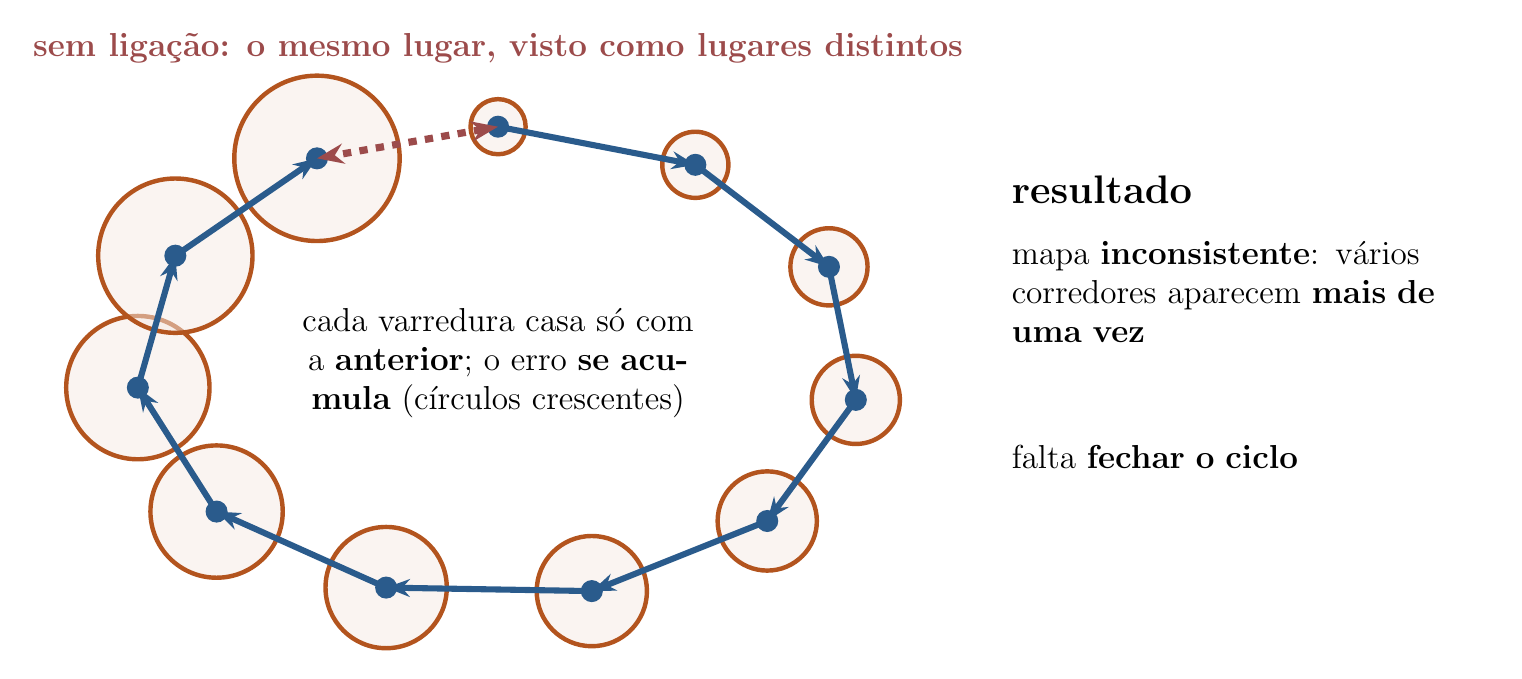
\begin{tikzpicture}[x=1cm,y=1cm]
\def\n{10}
\foreach \k in {0,...,\n} {
  \pgfmathsetmacro{\ang}{90-\k*33}
  \pgfmathsetmacro{\r}{0.10+\k*0.07}
  \coordinate (s\k) at ({6.0+4.6*cos(\ang)},{4.4+3.0*sin(\ang)});
  \draw[dorange, line width=1.6pt, fill=dorange!12, fill opacity=0.5] (s\k) circle (\r+0.25);
}
\foreach \k in {0,...,9} {\pgfmathtruncatemacro{\j}{\k+1}\draw[dblue, line width=2.2pt, -{Stealth[length=3mm]}] (s\k) -- (s\j);}
\foreach \k in {0,...,\n} {\fill[dblue] (s\k) circle (0.14);}
\draw[dred, line width=2.6pt, dashed, {Stealth[length=3.4mm]}-{Stealth[length=3.4mm]}] (s0) -- (s10);
\node[font=\large\bfseries, text=dred, fill=white, inner sep=2pt] at (6.0,8.4) {sem ligação: o mesmo lugar, visto como lugares distintos};
\node[font=\large, text width=7.0cm, align=center] at (6.0,4.4) {cada varredura casa só com a \textbf{anterior}; o erro \textbf{se acumula} (círculos crescentes)};
\node[font=\Large\bfseries, anchor=west] at (12.4,6.6) {resultado};
\node[font=\large, anchor=west, text width=6.0cm] at (12.4,5.3) {mapa \textbf{inconsistente}: vários corredores aparecem \textbf{mais de uma vez}};
\node[font=\large, anchor=west, text width=6.0cm] at (12.4,3.2) {falta \textbf{fechar o ciclo}};
\end{tikzpicture}
\end{document}
